%%%%%%%%%%%%%%%%%%%%%%%%%%%%%%%%%%%%%%%%%%%%%%%%%%%
%% P3: Phenomenology of Particle Physics                         
%%
%% Author:  André Rubbia                   		 
%%
%% Figure 20.2 Phase space for the Drell--Yan process
%%
%% This work is licensed under the Creative Commons Attribution 4.0 International License. 
%% To view a copy of this license, visit http://creativecommons.org/licenses/by/4.0/ or 
%% send a letter to Creative Commons, PO Box 1866, Mountain View, CA 94042, USA.
%%
%%%%%%%%%%%%%%%%%%%%%%%%%%%%%%%%%%%%%%%%%%%%%%%%%%%

\documentclass[a4paper,10pt]{article}

\usepackage[T1]{fontenc}
\usepackage[utf8]{inputenc}
\usepackage{lmodern}
\usepackage[labelfont=bf]{caption}
\usepackage{upgreek}

\usepackage{tikz}
\usepackage{pgfplots}
\pgfplotsset{compat=1.17}
\usepgfplotslibrary{ternary}
\usepgfplotslibrary{fillbetween}
\usepgfplotslibrary{external}

\def\d{\mathrm{d}}

\begin{document}

%%%%%%%%%%%%%%%%   FIGURE  %%%%%%%%%%%%%%%%%%%%%%%%%%%%%%
\begin{figure}[htb]
\centering
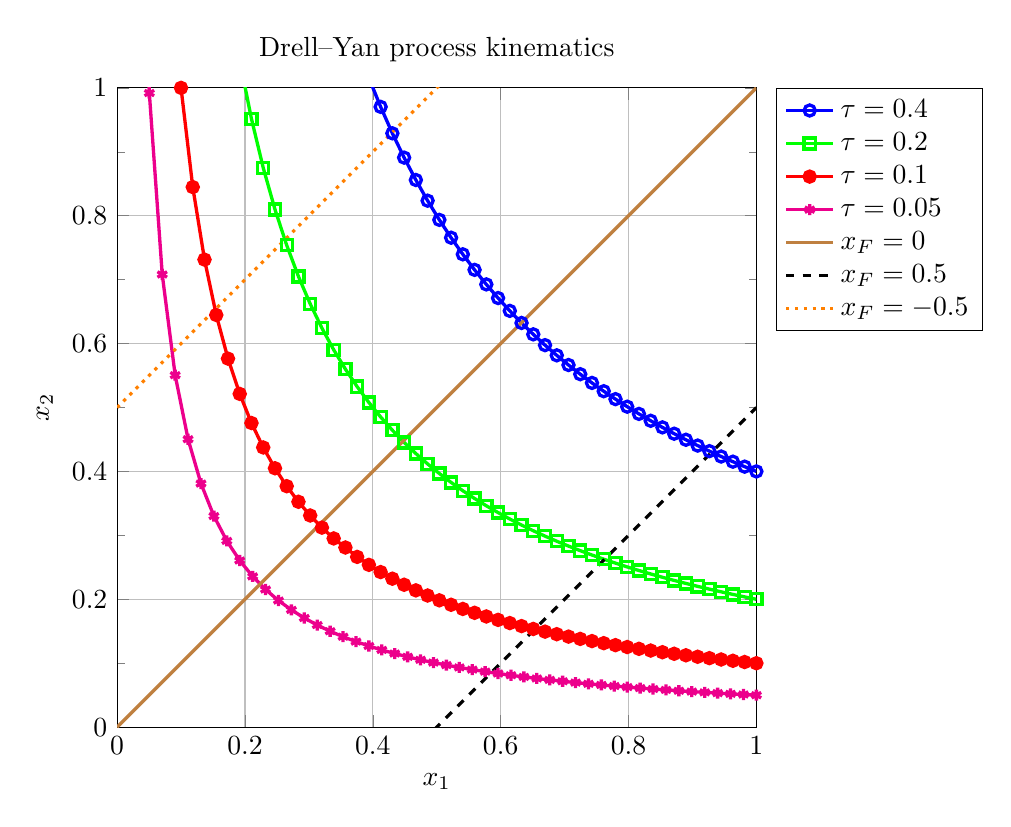
\begin{tikzpicture}[scale=1.]
    \begin{axis}[
    width=0.8\textwidth,
    height=0.8\textwidth,
        title=Drell--Yan process kinematics,
        xlabel={$x_1$},
        ylabel={$x_2$},
        xmin=0, xmax=1,
        ymin = 0, ymax=1,
        minor y tick num=1,
        grid = major,
	legend cell align = {left},
        legend entries={
        $\tau=0.4$,
        $\tau=0.2$,
        $\tau=0.1$,
        $\tau=0.05$,
        $x_F=0$,
        $x_F=0.5$,
        $x_F=-0.5$
        },
        legend style={legend pos = outer north east}
    ]
%  tau=0.4
        \addplot [blue,very thick,samples=50,domain=0.1:1, mark=o] {0.4/x};
%  tau=0.2
        \addplot [green,very thick,samples=50,domain=0.1:1, mark=square] {0.2/x};
%  tau=0.1
        \addplot [red,very thick,samples=50,domain=0.1:1, mark=*] {0.1/x};
%  tau=0.05
        \addplot [magenta,very thick,samples=50,domain=0.01:1,mark=asterisk] {0.05/x};
 %  x_f=0.0
        \addplot [brown,very thick, domain=0.0:1] {x-0};
 %  x_f=0.5
        \addplot [black,very thick,dashed, domain=0.0:1] {x-0.5};
 %  x_f=-0.5
        \addplot [orange,very thick, dotted, domain=0.0:1] {x+0.5};
  \end{axis}
\end{tikzpicture}%
\caption{Phase space for the Drell--Yan process. See the book for the definitions of $x_1$, $x_2$, $\tau$, and $x_F$.}
\end{figure}
%
%%%%%%%%%%%%%%%%   END FIGURE  %%%%%%%%%%%%%%%%%%%%%%%%%%%%%%
%
\end{document}
